\documentclass[12pt,a4paper,austrian]{article}
\usepackage{graphicx}
\usepackage[austrian, english]{babel}
\usepackage[utf8]{inputenc}
%\usepackage{listings}
\usepackage{multirow}
\usepackage{epstopdf}
\usepackage{amsmath}
\usepackage{amssymb} % fuer Mengen \N, Q, C, R
\usepackage{matlab-prettifier}
\graphicspath{{./fig/}}


%% Satzspiegel
\setlength{\hoffset}{-1in} \setlength{\textwidth}{18cm}
\setlength{\oddsidemargin}{1.5cm}
\setlength{\evensidemargin}{1.5cm}
\setlength{\marginparsep}{0.7em}
\setlength{\marginparwidth}{0.5cm}

\setlength{\voffset}{-1.9in}
\setlength{\headheight}{12pt}
\setlength{\topmargin}{2.6cm}
   \addtolength{\topmargin}{-\headheight}
\setlength{\headsep}{3.5cm}
   \addtolength{\headsep}{-\topmargin}
   \addtolength{\headsep}{-\headheight}
\setlength{\textheight}{27cm}

%% How should floats be treated?
\setlength{\floatsep}{12 pt plus 0 pt minus 8 pt}
\setlength{\textfloatsep}{12 pt plus 0pt minus 8 pt}
\setlength{\intextsep}{12 pt plus 0pt minus 8 pt}

\tolerance2000
\emergencystretch20pt

%% Text appearence
% English text
\newcommand{\eg}[1]%
  {\selectlanguage{english}\textit{#1}\selectlanguage{austrian}}

\newcommand{\filename}[1]
  {\begin{small}\texttt{#1}\end{small}}

\newcommand\IFT{\unitlength1mm\begin{picture}(10,2) \put (1,1)
{\circle{1.7}} \put(2,1){\line(1,0){5}} \put(8,1)
{\circle*{1.7}}\end{picture}}
\newcommand\FT{\unitlength1mm\begin{picture}(10,2) \put (1,1)
{\circle*{1.7}} \put(2,1){\line(1,0){5}} \put(8,1)
{\circle{1.7}}\end{picture}}

% A box for multiple choice problems
\newcommand{\choicebox}{\fbox{\rule{0pt}{0.5ex}\rule{0.5ex}{0pt}}}

\newenvironment{wahrfalsch}%
  {\bigskip\par\noindent\makebox[1cm][c]{richtig}\hspace{3mm}\makebox[1cm][c]{falsch}
   \begin{list}%
   {\makebox[1cm][c]{\choicebox}\hspace{3mm}\makebox[1cm][c]{\choicebox}}%
   {\setlength{\labelwidth}{2.31 cm}\setlength{\labelsep}{3mm}
    \setlength{\leftmargin}{2.61 cm}\setlength{\listparindent}{0pt}
    \setlength{\itemindent}{0pt}}%
  }
  {\end{list}}

\newcounter{theaufgabe}\setcounter{theaufgabe}{1}
\newenvironment{aufgabe}[1]%
  {\bigskip\par\noindent\begin{nopagebreak}
   \textsf{\textbf{Exercise \arabic{theaufgabe}}}\quad
      \textsf{\textit{#1}}\\*[1ex]%
\stepcounter{theaufgabe}\hspace{2ex}\end{nopagebreak}}
  {\par\pagebreak[2]}

% Innerhalb der Aufgaben erfolgt die weitere Unterteilung mittels einer
% enumerate Umgebung, die allerdings a), b),... zaehlen soll.
\renewcommand{\labelenumi}{\alph{enumi})}
\renewcommand{\labelenumii}{\arabic{enumii})}

% A box to tick for everything which has to done
\newcommand{\abgabe}{\marginpar{$\Box$}}
% Margin paragraphs on the left side
\reversemarginpar

% Language for listings
%\lstset{language=Vhdl,
%  basicstyle=\small\tt,
 % keywordstyle=\tt\bf,
 % commentstyle=\sl}

% No indention
\setlength{\parindent}{0.0cm}
% Don't number sections
\setcounter{secnumdepth}{0}

% prints a predefined preamble
% done this so that we don't have all the code later in the file
\newcommand{\printpreamble}{
  \pagestyle{plain}
  \thispagestyle{empty}
  \noindent
  \begin{minipage}[b][4cm]{1.0\textwidth}  
  \begin{center}
  \begin{bf} 
  \begin{large} Digital Signal Processing SS 2024 -- Exercise~2\end{large} \\
  \vspace{0.3cm}
  \begin{Large} Digital Signal Processing Tutorial  \end{Large} \\
  \vspace{0.3cm}
  \end{bf}
  \begin{large} 
  Group 23\\
  Aaron Zettler, 12105021\\
  Pascal Pilz, 12111234\\
  \end{large} 
  \end{center}
  \end{minipage}
  
  \noindent \rule[0.8em]{\textwidth}{0.12mm}\\[-0.5em]
}

%% Beginning of the text
%=======================================================================================

\begin{document}
\printpreamble

\begin{aufgabe}{} % Exercise 1 ---------------------------------------------------------

  \begin{enumerate}
    \item[(a)] We plot the discrete time signals in Matlab
    \begin{align*}
    x_1[n] &= -4 \delta[n+3]+4 \delta[n]-\delta[n-3]+2 \delta[n-7] & \text{for } -5 \leq n \leq 10 \\
    x_2[n] &= e^{-0.31 n} & \text{for } -5 \leq n \leq 10 \\
    x_3[n] &= 3 \sin \left(2 \pi \frac{3.5}{64} n\right) & \text{for } 0 \leq n \leq 256 \\
    x_4[n] &= -\cos \left(\frac{9}{64} n\right) & \text{for } 0 \leq n \leq 256
    \end{align*}
    
    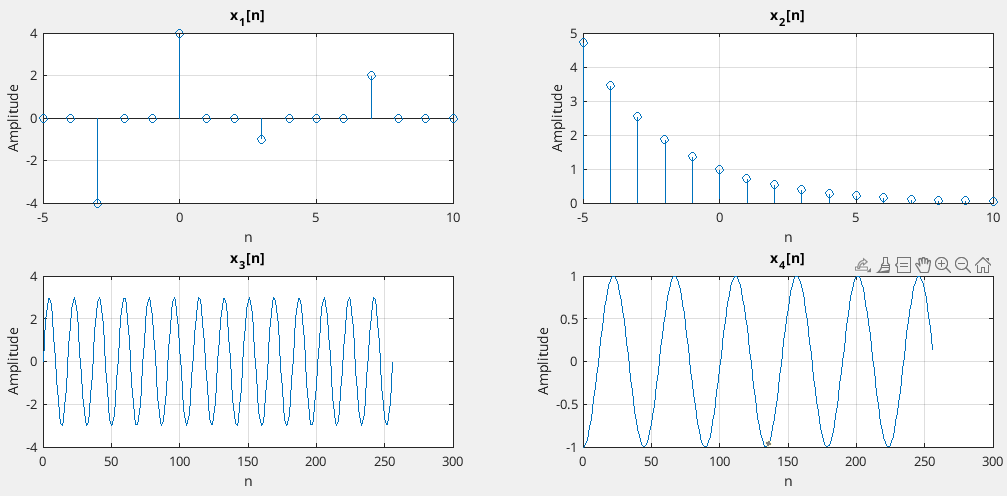
\includegraphics[width=0.7\textwidth]{../Ex01_a.png}
    
    \item[(b)] The normalized angular frequency $\Omega$: 
    For $x_3[n]$: $\Omega_{x3} = 0.3436$ and for $x_4[n]$: $\Omega_{x4} = 0.1406$:   
    
    \item[(c)] The signals $x_3[n]$ and $x_4[n]$ are periodic with fundamental periods $T_{x3} = 18.2857$ \\
               and $T_{x4} = 44.6804$, respectively.
    
    \item[(d)] The powers for the periodic signals $x_3[n]$ and $x_4[n]$ are $P_{x3} = 4.5658$ and $P_{x4} = 0.4925$.
    
    \item[(e)] The energies according to $W=\sum_{n=-\infty}^{\infty}|x[n]|^2$ for these time-limited signals  \\
               $W_{x1} = 37$, $W_{x2} = 48.0394$, $W_{x3} = 1152$ and $W_{x4} = 128.9565$.
    
    \item[(f)] All signal powers of (d) and signal energies of (e) in a single table.
    \begin{table}[htbp]
        \centering
        \begin{tabular}{|c|c|c|}
            \hline
            Signal & Power ($P$) & Energy ($W$) \\
            \hline
            $x_1[n]$ & X & 37 \\
            $x_2[n]$ & X & 48.0394 \\
            $x_3[n]$ & 4.5658 & 1152 \\
            $x_4[n]$ & 0.4925 & 128.9565 \\
            \hline
        \end{tabular}
    \end{table}
\end{enumerate}

  

\end{aufgabe} \pagebreak

\begin{aufgabe}{} % Exercise 2 ---------------------------------------------------------
  The signal $x[n]=(3,-1,2,0,1)$ at sample times $n=(0,1,2,3,4)$ is the input to an LTI system with impulse response $h[n]=(2,3,4,1)$ at sample times $n=(0,1,2,3)$.
  \begin{enumerate}
    \item[(a)] We calculate the length of the output signal $y[n]$: \bigskip
    \begin{enumerate}
      \item We know (DSP\_04 page 15): \\
      If $x[n]$ and $h[n]$ have finite lengths $N_x$ and $N_h$ respectively, \\
      then the length of the output signal $y[n]$ is given by $N_y=N_x+N_h-1$. \bigskip

      \item So with $N_x=5$ and $N_h=4$ we get: $N_y=5+4-1=8$.

    \end{enumerate}

    \item[(b)] We calculate the output signal $y[n]$ manually:

    \begin{enumerate}
      \item We know the formula for convolution (DSP\_04 page 17): $y[n] = \sum_{i=0}^{\infty} x[i] \cdot h[n-i]$

      \item Given $x[n] = (3, -1, 2, 0, 1)$ \& $h[n] = (2, 3, 4, 1)$, we find the output signal $y[n]$ for each $n$:

      \begin{align*}
        \text{For n=0:}  &\quad y[0] = x[0] \cdot h[0] = 3 \cdot 2 = 6 \\
        \text{For n=1:}  &\quad y[1] = x[0] \cdot h[1] + x[1] \cdot h[0] = 3 \cdot 3 + (-1) \cdot 2 = 7 \\
        \text{For n=2:}  &\quad y[2] = x[0] \cdot h[2] + x[1] \cdot h[1] + x[2] \cdot h[0] \\
                         &\quad = 3 \cdot 4 + (-1) \cdot 3 + 2 \cdot 2 = 12 - 3 + 4 = 13 \\
        \text{For n=3:}  &\quad y[3] = x[0] \cdot h[3] + x[1] \cdot h[2] + x[2] \cdot h[1] + x[3] \cdot h[0] \\
                         &\quad = 3 \cdot 1 + (-1) \cdot 4 + 2 \cdot 3 + 0 \cdot 2 = 3 - 4 + 6 + 0 = 5 \\
        \text{For n=4:}  &\quad y[4] = x[1] \cdot h[3] + x[2] \cdot h[2] + x[3] \cdot h[1] + x[4] \cdot h[0] \\
                         &\quad = (-1) \cdot 1 + 2 \cdot 4 + 0 \cdot 3 + 1 \cdot 2 = -1 + 8 + 0 + 2 = 9 \\
        \text{For n=5:}  &\quad y[5] = x[2] \cdot h[3] + x[3] \cdot h[2] + x[4] \cdot h[1] = 2 \cdot 1 + 0 \cdot 4 + 1 \cdot 3 = 2 + 0 + 3 = 5 \\
        \text{For n=6:}  &\quad y[6] = x[3] \cdot h[3] + x[4] \cdot h[2] = 0 \cdot 1 + 1 \cdot 4 = 0 + 4 = 4 \\
        \text{For n=7:}  &\quad y[7] = x[4] \cdot h[3] = 1 \cdot 1 = 1 \\
    \end{align*}
    
    \item So, the output signal $y[n]$ is $(6, 7, 13, 5, 9, 5, 4, 1)$.
    \end{enumerate}
  \end{enumerate}
\end{aufgabe} \pagebreak

\begin{aufgabe}{} % Exercise 3 ---------------------------------------------------------

  We have the impulse response of an LTI system $h[n] = (0.25 , 0.5 , 0.25)$ at sample indices $n = (0,1,2)$. The input signal is $x[n] = \cos \left( \frac{2 \pi}{20} n \right)$ for $0 \leq n < 50$.

  \begin{enumerate}
    \item From the lecture: If $x[n]$ and $h[n]$ have finite lengths $N_x$ and $N_h$, the length of the output signal results to $N_y = N_x + N_h - 1$. In our example we have $N_x = 50$ and $N_h = 3$, therefore we can calculate the length of the output signal $L_y$ ($N_y$ in the lecture) as $\underline{L_y = 52}$.
    
    \item For the actual implementation, see code \texttt{Ex03.m}. Here it was important to explicitly define $x[n]$ to be 0 outside the given range.
    
    \item 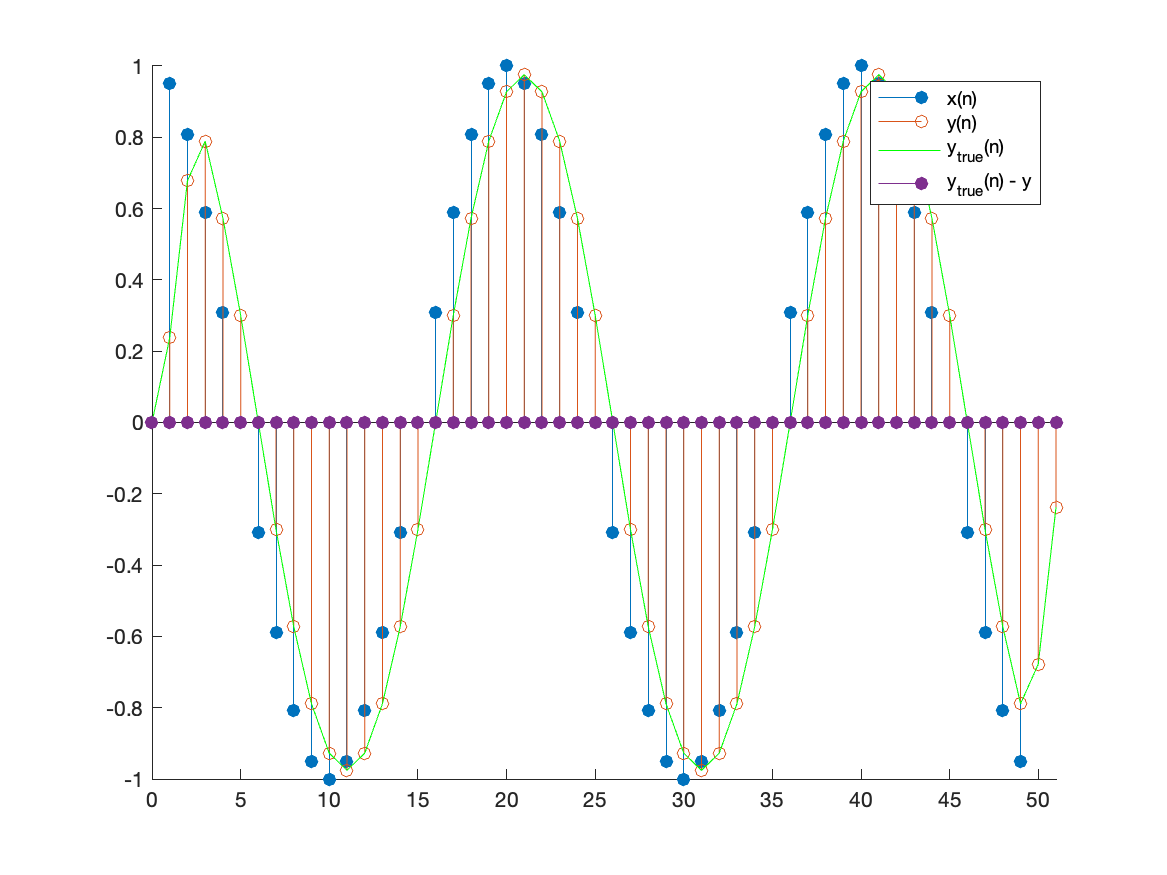
\includegraphics[width=0.9\textwidth]{../Ex03.png}
    
    \item As we can see in the plot, the "true" $y$ and our calculated $y$ match up.
  \end{enumerate}

\end{aufgabe} \pagebreak

\begin{aufgabe}{} % Exercise 4 ---------------------------------------------------------

  \begin{enumerate}
    \item See \texttt{Ex04.m} for the full code, here I show only the function \texttt{dtft}:
    \begin{lstlisting}[style=Matlab-editor]
function X = dtft(x, n, w)
    % DTFT Computes Discrete-time Fourier transform
    % @param    x: finite duration sequence over n
    % @param    n: sample position vector
    % @param    w: frquency location vector
    % @return   X: DTFT values computed at w frequencies

    X = x * exp(-1j .* n' * w);

end
    \end{lstlisting}
    We call the function via \texttt{X = dtft(@x, n, w)}, where
    \begin{itemize}
      \item \texttt{x(n) = ((0.8).\string^abs(n)) .* (u(n+10) - u(n-11))} with \texttt{u(n) = 1.*(n>=0)}
      \item \texttt{n = -10:10}
      \item \texttt{w = linspace(Omega * -pi, Omega * pi, 1000)} for \texttt{Omega = 1}
    \end{itemize}

    \item What I can observe on the y-axis of the phase response plot is that the phase response for the settings described above is very small, in fact less than $10^{-14}$.
    
    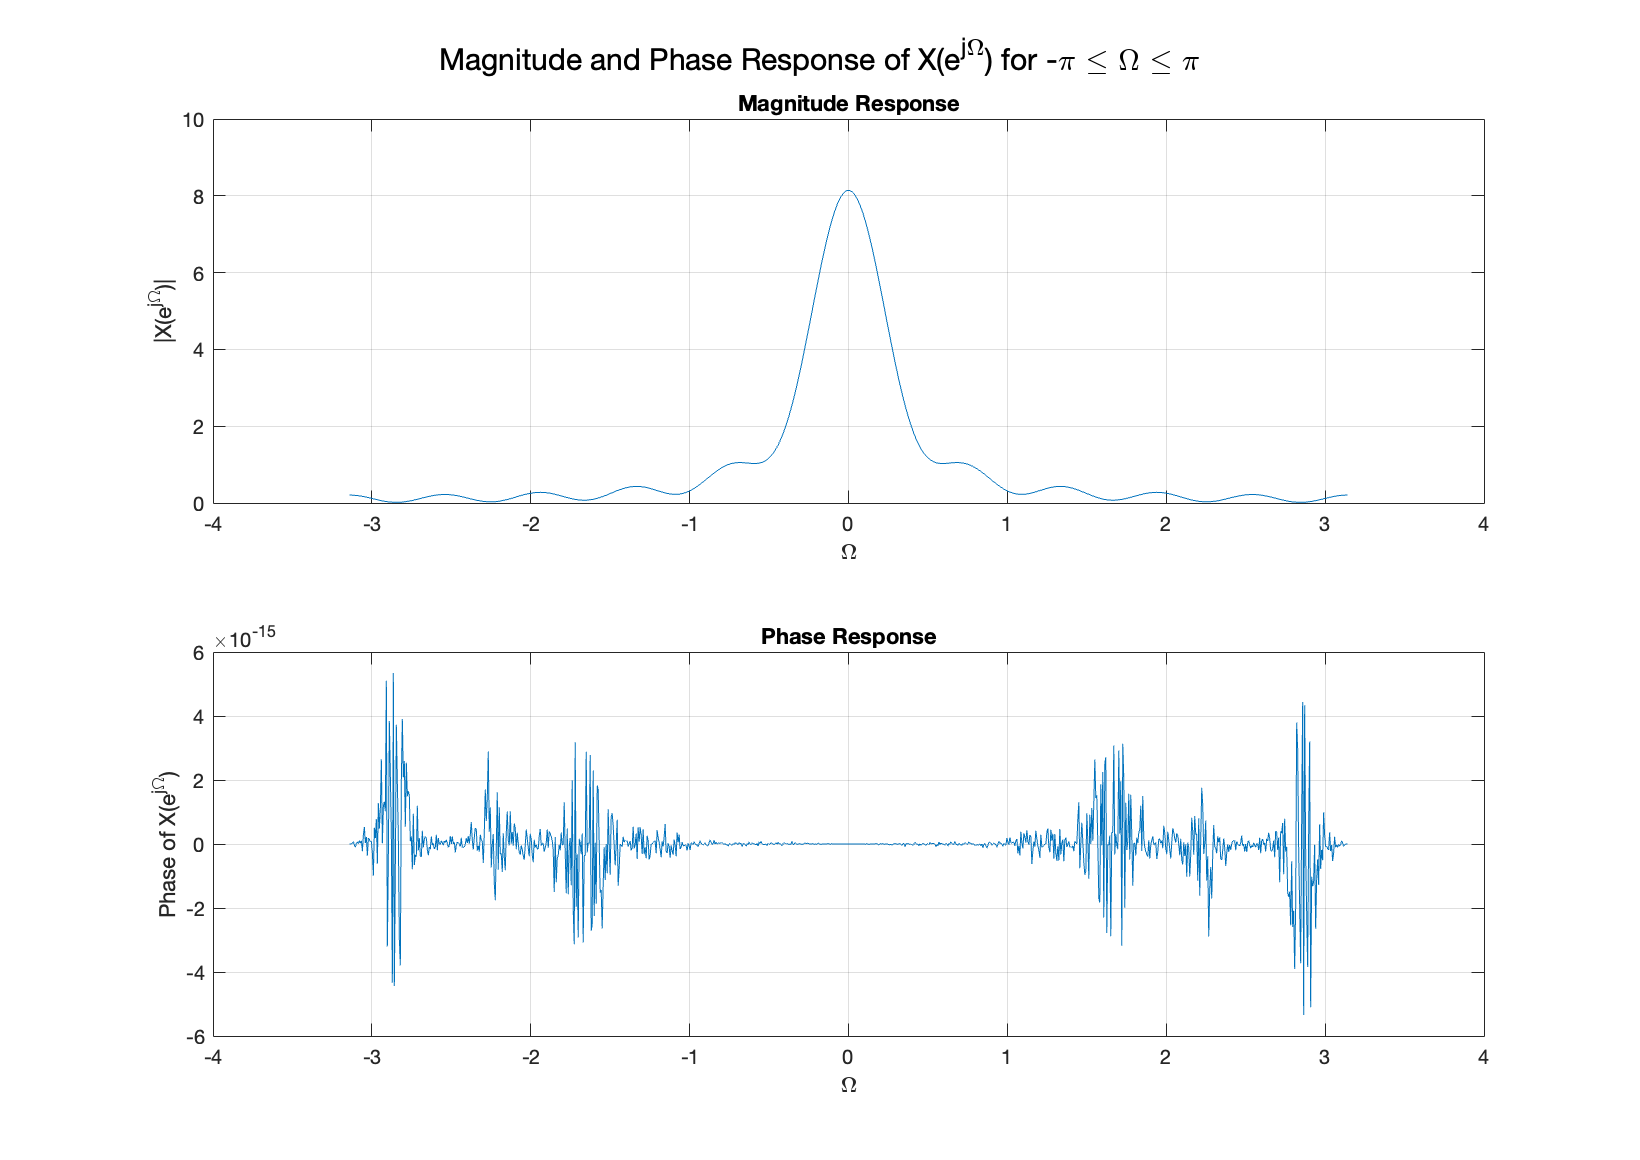
\includegraphics[width=0.9\textwidth]{../Ex04_b.png}

    \item If we change \texttt{Omega} from \texttt{Omega = 1} to \texttt{Omega = 5}, we can see that the magnitude response has peaks and troughs at multiples of $\pi$. We can also see that the phase response seems to be mirrored and flipped around the y-axis (graphic on next page).
    
    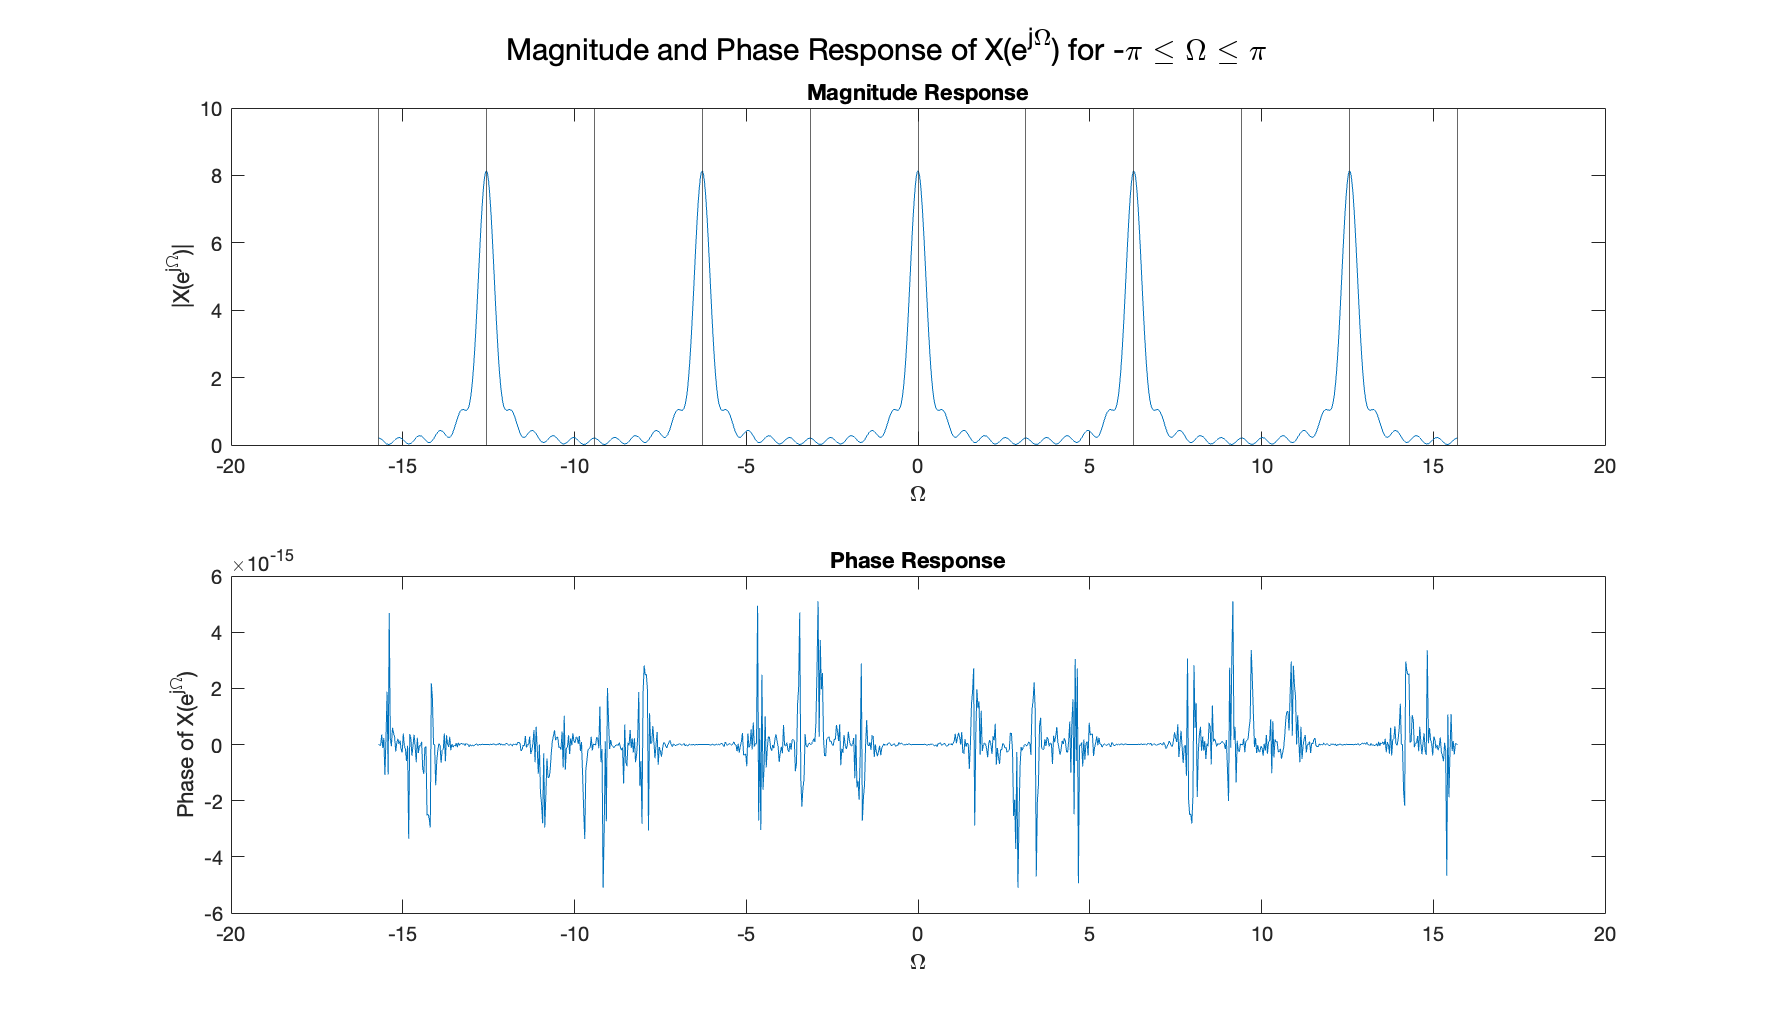
\includegraphics[width=0.9\textwidth]{../Ex04_c.png}

  \end{enumerate}

\end{aufgabe} \pagebreak

\end{document}
